% Created 2014-12-06 Sat 13:29
\documentclass[presentation]{beamer}
\usepackage[utf8]{inputenc}
\usepackage[T1]{fontenc}
\usepackage{fixltx2e}
\usepackage{graphicx}
\usepackage{longtable}
\usepackage{float}
\usepackage{wrapfig}
\usepackage{rotating}
\usepackage[normalem]{ulem}
\usepackage{amsmath}
\usepackage{textcomp}
\usepackage{marvosym}
\usepackage{wasysym}
\usepackage{amssymb}
\usepackage{hyperref}
\tolerance=1000
\usetheme{default}
\usecolortheme{spruce}
\author{Üstün Özgür}
\date{\today}
\title{Postgresql: Web Programcısı için Gündelik İpuçları \\ Postgres 2014 Türkiye}
\hypersetup{
  pdfkeywords={},
  pdfsubject={},
  pdfcreator={Emacs 24.4.1 (Org mode 8.2.10)}}
\begin{document}

\maketitle
\begin{frame}{Outline}
\tableofcontents
\end{frame}


\begin{frame}[label=sec-1]{Giriş}
\begin{itemize}
\item Web uygulama çatıları (frameworkler)

\item MVC
\begin{itemize}
\item Java Spring + Hibernate, Python Django, Ruby Rails
\end{itemize}
\item ORM (Nesne-İlişkisel Dönüşümü)
\begin{itemize}
\item Bu dönüşüm esnasında yaşanan impedance mismatch
\end{itemize}
\item Veritabanından uzak geliştiriciler
\item Veritabanı uygulamanın en önemli parçalarından biri, belki de en önemlisi
\item Web programlaması için önemli Postgres kavramları ve ipuçları
\end{itemize}
\end{frame}

\begin{frame}[label=sec-2]{SQL Bir Programlama Dilidir}
\begin{itemize}
\item Temelde bir sorgulama dili
\item ilk bakışta göründüğünden daha güçlü bir dil: Turing complete!
\item Sadece tablolar değil: fonksiyonlar ve diğer expressionlar
\item Nasıldan çok neyi istediğimizi söylediğimiz deklaratif bir dil
\end{itemize}
\end{frame}

\begin{frame}[fragile,label=sec-3]{Basit Bir Örnek}
 \begin{itemize}
\item \texttt{SELECT sin(pi()/4);}
\item \texttt{SELECT generate\_series(1,8)}
\item \texttt{SELECT sin(2*pi()/i) from generate\_series(1,8) as i;}
\end{itemize}
\end{frame}



\begin{frame}[label=sec-4]{Bir Programlama Dili Olarak SQL}
\begin{itemize}
\item İlişkiler üzerinde operasyonlar
\item Genelde sütun bazında operasyonlar: Yüksek seviye fonksiyonlar
\item Yanlış bir tabir de olsa SQL için fonksiyonel diyebiliriz
\item Üç temel yüksek seviye fonksiyon: Map, Filter, Reduce
\item SQL hepsini sağlıyor.
\end{itemize}
\end{frame}

\begin{frame}[fragile,label=sec-5]{Map, Filter, Reduce}
 \begin{itemize}
\item Map \texttt{SELECT foo(x) from table};
\item foo fonksiyonunu bütün x değerleri için uygula
\item \texttt{SELECT foo(x) from table where predicate(x)} dediğimizde
\end{itemize}
filter'a denk şekilde bir predicate fonksiyonu uygular. (Predicate fonksiyon
boolean dönen fonksiyon)
\begin{itemize}
\item Eğer foo aggregate yapıda bir fonksiyon ise de reduce'a denktir diyebiliriz.
\end{itemize}
\end{frame}

\begin{frame}[fragile,label=sec-6]{Örnek: Faktoriyel Implementasyonu (1/2)}
 \begin{verbatim}
select generate_series(1, 10);
select generate_series(1, 10, 2);
select 3 * 4;
select numeric_mul(3, 4);
\end{verbatim}
\end{frame}

\begin{frame}[fragile,label=sec-7]{Örnek: Faktoriyel Implementasyonu (2/2)}
 \begin{verbatim}
create aggregate product(numeric) (sfunc=numeric_mul, stype=numeric, initcond=1);
select product(x) from generate_series(1, 5) as x;

create function myfactorial(i numeric)
   returns integer
   as 'select product(x)
        from generate_series(1, i::integer) as x;'
   language sql;
\end{verbatim}
\end{frame}

\begin{frame}[fragile,label=sec-8]{Trivia: Postgresql'de kac tane fonksiyon vardir?}
 \begin{verbatim}
\df
\set ECHO_HIDDEN
\end{verbatim}
\end{frame}

\begin{frame}[fragile,label=sec-9]{psql}
 \begin{itemize}
\item "In the beginning, there was the command line."
\item GUI'leri tercih etseniz de ogrenilmesi cok yararli
\item Kolay denemeler, SQL pratigi
\item En önemli psql komutları:
\begin{itemize}
\item \texttt{\textbackslash{}h} : SQL komutlari hakkinda bilgi
Or: \texttt{\textbackslash{}h CREATE TABLE}
\item \texttt{\textbackslash{}?} : psql komutlari hakkinda bilgi
\end{itemize}
\end{itemize}
\end{frame}

\begin{frame}[fragile,label=sec-10]{psql demo}
 \begin{verbatim}
\h
\h CREATE
\h CREATE TABLE
\h ALTER TRIGGER
\end{verbatim}

\begin{itemize}
\item Psql'a ait özel komutlar $\backslash$ ile başlar
\end{itemize}
\end{frame}

\begin{frame}[fragile,label=sec-11]{psql komutlari demo}
 \begin{verbatim}
| \l       | Bütün veritabanlari     |
| \d       | Bütün tablolar, viewlar |
| \d+      | Daha ayrıntılı bilgi    |
| \df      | Kullanıcı Fonksiyonları |
| \dfS     | Sistem fonksiyonlari    |
| \dft     | Triggerlar              |
| show all | Bütün ayarlar           |
| \e       | Edit                    |
| \o       | Çıktı dosyası belirleme |
| \H       | HTML tablo çıktısı      |
\end{verbatim}


\texttt{\textbackslash{}!  make\_pretty\_table foo.html}
\end{frame}


\begin{frame}[fragile,label=sec-12]{.psqlrc dosyasi}
 \begin{itemize}
\item Bu komutlar başlangıçta çalıştırılacaktır.
\end{itemize}

\begin{verbatim}
\x auto
\timing
\end{verbatim}

\begin{itemize}
\item \texttt{Ctrl-r} ile shell'deki gibi eski komutlar arasında arama
\end{itemize}
yapabiliriz.
\end{frame}

\begin{frame}[fragile,label=sec-13]{Performans ipuçları (1/4)}
 \begin{itemize}
\item Sayfalarınızda toplamda kaç tane SQL sorgusunun gösteren bir araç kullanın.
\item Örneğin Django için django-debug-toolbar.
\item \texttt{./manage.py shell\_plus -{}-print-sql}
\item psql'de \texttt{\textbackslash{}timing} kullanımı
\item \texttt{ANALYZE} ve \texttt{EXPLAIN ANALYZE} komutu ve index ekleme
\item \texttt{log\_collector} ile yapilan SQL sorgularinin ve sürelerinin kaydedilmesi
\end{itemize}
\end{frame}

\begin{frame}[fragile,label=sec-14]{Performans ipuçları (2/5)}
 \begin{itemize}
\item ORM'lerde olabilecek en büyük sorun N+1 sorguları.
\item Örneğin N tane soru göstereceksiniz, bu soruları soran kişinin de ismini
göstereceksiniz.
\item N+1 tehlikesine çok müsait.
\item Django için \texttt{select\_related} ve \texttt{prefetch\_related}
\end{itemize}
\end{frame}

\begin{frame}[label=sec-15]{Performans ipuçları (3/5)}
\begin{itemize}
\item Bağlantı havuzu: Bağlantıların kurulması çok fazla zaman alabilir.
\item pgbouncer gibi bir bağlantı havuzu sağlayın. Kurulması oldukça kolay.
\item pgtune uygulaması: Postgres'in default konfigürasyonu oldukça verimsiz
\item Sessionları veritabanında tutmak yerine redis'te tutmak
\end{itemize}
\end{frame}

\begin{frame}[label=sec-16]{Performans ipuçları (4/5)}
\begin{itemize}
\item Makineye göre optimize etmek için \url{https://github.com/gregs1104/pgtune}
\item Web versiyonu \url{http://pgtune.leopard.in.ua/}
\end{itemize}

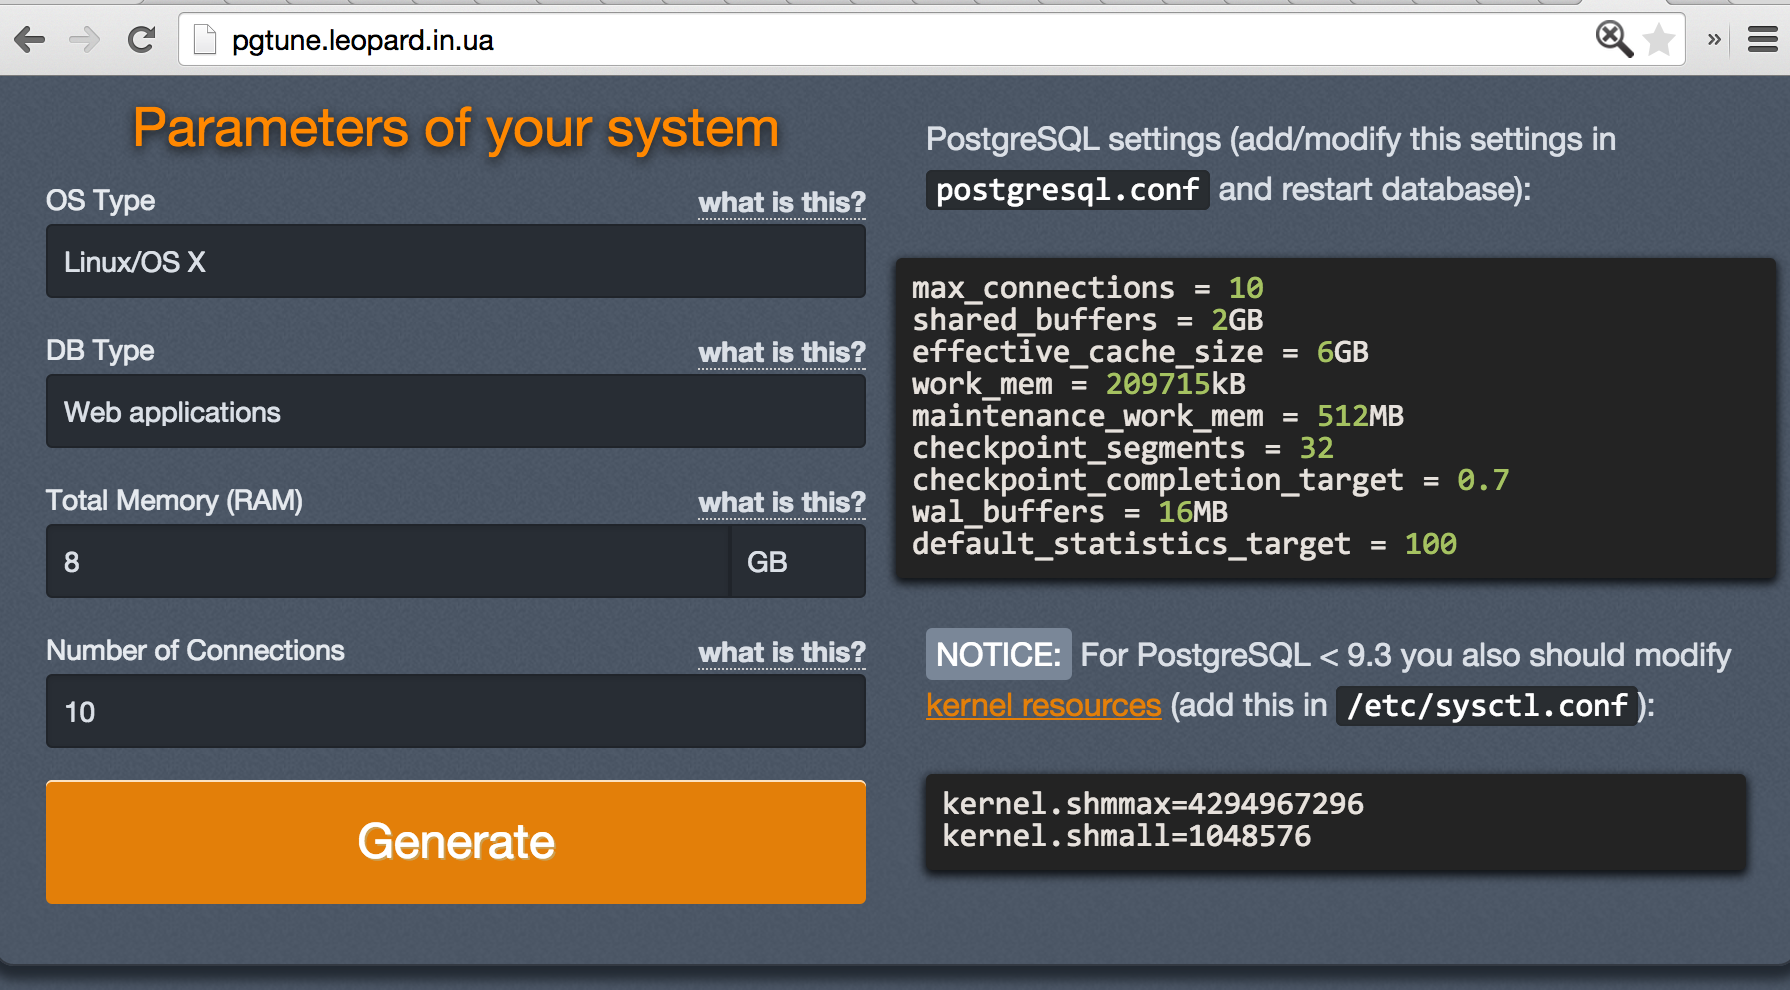
\includegraphics[width=.9\linewidth]{./pgtune.png}
\end{frame}


\begin{frame}[fragile,label=sec-17]{Performans ipuçları (5/5)}
 \begin{itemize}
\item Pghero: \url{https://github.com/ankane/pghero}
\begin{itemize}
\item \texttt{SELECT * FROM pghero\_missing\_indexes;}
\item \texttt{SELECT * FROM pghero\_relation\_sizes;}
\item \texttt{SELECT pghero\_index\_hit\_rate();}
\item \texttt{SELECT * FROM pghero\_unused\_indexes;}
\end{itemize}
\item Monitoring için NewRelic ya da AppNeta gibi araçlar da production esnasında
performans sorunlarını takip etmek için kullanılabilir. Bu araçların kurulumu
oldukça zahmetsiz.
\end{itemize}
\end{frame}

\begin{frame}[fragile,label=sec-18]{Yedekler (Geliştirme)}
 \begin{itemize}
\item Development esnasında hızlıca yedek almak için

\item \texttt{CREATE DATABASE foo with TEMPLATE bar;}
\end{itemize}
\end{frame}

\begin{frame}[fragile,label=sec-19]{Yedekler (Geliştirme)}
 \begin{verbatim}
DB_NAME=mydb
echo "SELECT pg_terminate_backend(pid)
   FROM pg_stat_activity WHERE pid <>
   pg_backend_pid() AND datname = '${DB_NAME}';" | psql
echo "create database
   ${DB_NAME}_$(date '+%Y%m%d_%H%M%S')
   with template ${DB_NAME}" | psql
\end{verbatim}
\end{frame}

\begin{frame}[fragile,label=sec-20]{Yedekler (Production'da)}
 \begin{itemize}
\item En azından \texttt{pg\_dump} ile günlük backuplar alın ve başka bir makineye (S3 vs.) gönderin.
\item Streaming replication yapabilirsiniz, son Postgres sürümlerinde bu oldukça
kolaylaştı
\item Josh Berkus'un "Ten Minutes to Replication" sunumu
\item \url{http://www.youtube.com/watch?v=BD7i9QImqic}
\end{itemize}
\end{frame}


\begin{frame}[label=sec-21]{NoSQL desteği}
\begin{itemize}
\item Postgres bir object-relational veritabanıdır.
\item Object-relational?
\item Extended relational
\item Postgres'in tasarımının anlatıldığı ilk makale Stonebreaker
\item Postgres'in ilk hedefi olarak ilişkisel veritabanlarının yetersiz ya da düşük
performanslı kaldığı noktaları vurgulamaktadır.
\end{itemize}
\end{frame}

\begin{frame}[label=sec-22]{Örnek Uygulama}
\begin{itemize}
\item Bir Kullanıcı-Adres ilişkisi
\item Her kullanıcının tek bir adresi olsun
\item Adresin de kendi içinde birden fazla alanı olsun, örneğin şehir ve posta kodu gibi.

\item Normalize edilmiş bir veritabanında iki ayrı tablo
\item Çoğu zaman doğru çözüm
\item Bazen farklı bir çözüm gerekir: Aynı tabloda tutmak
\end{itemize}
\end{frame}

\begin{frame}[fragile,label=sec-23]{Farklı Çözümler}
 \begin{itemize}
\item Çözüm 1:
\begin{itemize}
\item Kullanıcı tablosuna şehir ve posta kodu alanları eklenebilir
\item Çok fazla alan
\end{itemize}
\item Çözüm 2:
\begin{itemize}
\item adres bilgisinin bir metne dönüştürülmesi
\item zor veri sorgulaması, \texttt{LİKE} veya regular expression kullanımı
\end{itemize}
\end{itemize}
\end{frame}

\begin{frame}[fragile,label=sec-24]{Composite Types}
 \begin{itemize}
\item Tek bir alanda birden fazla veri saklamak için
\item Her tablo için bir de type üretir
\item Kendimiz de type tanımlayabiliriz
\end{itemize}

\begin{verbatim}
create type adres as (sehir text, posta_kodu text);
create table myuser  (id int primary key, adres adres,
                      isim text);

insert into myuser(id, adres, isim) values(1,
     ('Ankara', '06370')::adres, 'Ustun');

select * from myuser where (adres).sehir='Ankara';
\end{verbatim}
\end{frame}

\begin{frame}[label=sec-25]{hstore ve json}
\begin{itemize}
\item hstore ve json
\item 9.4'te jsonb (binary json)
\item Alan adları esnek
\item hstore ile json'un temel farki ise hstore'un sadece tek seviye ilişkiye izin
vermesi
\end{itemize}
\end{frame}

\begin{frame}[label=sec-26]{hstore}
\begin{itemize}
\item Demo
\end{itemize}
\end{frame}

\begin{frame}[label=sec-27]{json}
\begin{itemize}
\item Demo
\end{itemize}
\end{frame}

\begin{frame}[label=sec-28]{Array}
\begin{itemize}
\item Demo
\end{itemize}
\end{frame}

\begin{frame}[label=sec-29]{Soyutlamalar}
\begin{itemize}
\item Views
\item Materialized Views
\end{itemize}
\end{frame}

\begin{frame}[fragile,label=sec-30]{Views}
 \begin{itemize}
\item Gerçek tablo değil
\item Bir query'ye isim verip soyutlamak
\item Örneğin Kullanıcı tablomuzda aktif olup olmadığını gösteren bir
\end{itemize}
sütun olsun.
\begin{itemize}
\item \texttt{SELECT * FROM Kullanici WHERE active=t}
\item \texttt{CREATE VIEW AktifKullanici AS SELECT * FROM Kullanici WHERE active=t;}
\item \texttt{SELECT * From AktifKullanıcı}
\item SQL'e göre güzel bir özelliği daha composable olmasıdır
\item Örnek: son hafta eklenmiş aktif kullanıcılar
\item \texttt{SELECT * FROM AktifKullanici WHERE tarih\_eklenme > now() - '1 week'::interval;}
\item Zincirleme
\end{itemize}
\end{frame}

\begin{frame}[label=sec-31]{Daha Mantıklı Bir View Örneği}
\begin{itemize}
\item Kütüphane uygulaması
\item Kullanıcılar ve Kitaplar
\item Ödünç alınan kitaplar tablosu
\item Normalize olursa sadece kullanıcı ve kitap id'lerini görebiliriz
\item Kullanıcı adı ve ödünç aldıkları kitapları görmek için bir view yazalım.
\end{itemize}
\end{frame}

\begin{frame}[fragile,label=sec-32]{Örneğe Devam}
 \begin{verbatim}
create table kutuphane_kullanici (id serial primary key, name text);
create table kutuphane_kitap (id serial primary key, name text);
create table kutuphane_odunc_kitaplar
   (id serial primary key,
   kullanici_id int references kutuphane_kullanici,
   kitap_id int references kütüphane_kitap);
\end{verbatim}
\end{frame}

\begin{frame}[fragile,label=sec-33]{Örneğe Devam}
 \begin{verbatim}
insert into kutuphane_kullanici(name) values ('Üstün'), ('Ahmet');
insert into kutuphane_kitap(name) values ('Anna Karenina'), ('Karamazov Kardeşler');
insert into kutuphane_odunc_kitaplar values (1,1), (2,2);
\end{verbatim}
\end{frame}

\begin{frame}[fragile,label=sec-34]{Örneğe Devam}
 \begin{verbatim}
# select * from kutuphane_odunc_kitaplar;
 id | kullanici_id | kitap_id
----+--------------+----------
  1 |            1 |   1
  2 |            2 |   2
# select k.name, ki.name from kutuphane_odunc_kitaplar o,
 kutuphane_kullanici k,  kutuphane_kitap ki
 where o.kullanici_id=k.id and ki.id=kitap_id;
 name  |        name
-------+---------------------
 Ustun | Anna Karenina
 Ahmet | Karamazov Kardesler
(2 rows)
\end{verbatim}
\end{frame}

\begin{frame}[fragile,label=sec-35]{Örneğe Devam}
 \begin{verbatim}
# select k.name as KullaniciAdi, ki.name as KitapAdi
from kutuphane_odunc_kitaplar o, kutuphane_kullanici k, kutuphane_kitap ki
 where o.kullanici_id=k.id and ki.id=kitap_id;
 kullaniciadi |      kitapadi
--------------+---------------------
 Ustun        | Anna Karenina
 Ahmet        | Karamazov Kardesler
(2 rows)

Time: 1.296 ms
\end{verbatim}
\end{frame}

\begin{frame}[fragile,label=sec-36]{Örneğe Devam}
 \begin{verbatim}
# create view OduncKitaplar as select k.name as KullaniciAdi,
ki.name as KitapAdi from kutuphane_odunc_kitaplar o,
kutuphane_kullanici k, kutuphane_kitap ki
 where o.kullanici_id=k.id and ki.id=kitap_id;
CREATE VIEW
Time: 7.588 ms
# select * from OduncKitaplar;
 kullaniciadi |      kitapadi
--------------+---------------------
 Ustun        | Anna Karenina
 Ahmet        | Karamazov Kardesler
(2 rows)
\end{verbatim}
\end{frame}

\begin{frame}[label=sec-37]{Materialized Views}
\begin{itemize}
\item 9.3
\item Sorgu sonuçları gerçek tablolarda saklanır
\item Otomatik güncelleme şu an yok
\item Periyodik olarak ya da bir trigger sonrasında elle güncelleme
\end{itemize}
\end{frame}

\begin{frame}[label=sec-38]{Trigger ve Audit Tabloları}
\begin{itemize}
\item Yapılan her INSERT, UPDATE, DELETE sonrası bir işlem çalıştırmak
\item Audit tablosu: Önemli tablolara ek bir tablo. Yapılan işlemin kaydını
tutuyor.
\item Hatalı veri kaydına karşı bir koruma sağlar
\end{itemize}
\end{frame}

\begin{frame}[label=sec-39]{Yararlanabileceginiz Kaynaklar}
\begin{itemize}
\item Resmi dokumanlar harika
\item Postgres Weekly
\item postgres guide
\item postgres planet
\item kitaplar: High Performance Postgres
\end{itemize}
\end{frame}


\begin{frame}[label=sec-40]{Teşekkürler}
\begin{itemize}
\item ustun@ustunozgur.com
\item \url{https://github.com/ustun/postgres-2014}
\end{itemize}
\end{frame}
% Emacs 24.4.1 (Org mode 8.2.10)
\end{document}
